%% TRABALHO DE CONCLUSAO DE CURSO UGF - PIEDADE
%%%%%%%%%%%%%%%%%%%%%%%%%%%%%%%%%%%%%%%%%%%%%%%%%%%%%%%%%%%%%%%%%%%%%%%%%%%%%

\documentclass[a4paper,12pt]{abnt-UTFPR} % estilo de documento abnTeX
\usepackage[alf,abnt-emphasize=bf,bibjustif,recuo=0cm]{abntcite} % estilo de bibliografia abnTeX
\usepackage[brazil]{babel} % pacote portugues brasileiro
\usepackage{setspace}
\usepackage{amsmath,amsfonts,amssymb} % pacote matematico
\usepackage{graphicx} % pacote grafico
\usepackage[utf8]{inputenc}
\usepackage[brazil]{varioref}
\renewcommand{\rmdefault}{phv} % Arial
\renewcommand{\sfdefault}{phv} % Arial

\usepackage{xspace}
\usepackage{color}
\usepackage{xcolor}
\usepackage{subfigure}
\usepackage{xtab}
\usepackage{nomencl}
\usepackage[portuguese,algoruled,longend,linesnumbered]{algorithm2e}

\usepackage{makeidx}
\makeindex


% ---------- Preambulo ----------
\instituicao{UGF - Universidade Gama Filho} % nome da instituicao

\titulo{TÍTULO} % titulo do trabalho

\autor{AUTOR 1} % nome do autor 1
\autorU{AUTOR 2} % nome do autor 2

\palavraschave{palavra chave} % palavras-chave do trabalho
\keywords{palavra chave em inglês} % palavras-chave do trabalho em ingles

\comentario{Trabalho de Conclus\~ao de curso apresentado como requisito obrigat\'orio para obten\c{c}\~ao do t\'itulo de Bacharel em Ci\^encia da Computa\c{c}\~ao da UGF - Universidade Gama Filho.}

\orientador{Orientador} % nome do orientador do trabalho
\coorientador[Co-orientadora:]{\hspace{1.2mm}{Coorientador se tiver, senão comente a linha}} % <- no caso de co-orientadora, usar esta sintaxe

\local{Rio de Janeiro} %cidade
\data{2013} %ano

%-----------------------INÍCIO DO DOCUMENTO ----------------------
\begin{document}

%------------------------CAPA DO DOCUMENTO------------------------
\capa 
%--------------------FOLHA DE ROSTO DO DOCUMENTO------------------
\folhaderosto
% -----------------------TERMO DE APROVAÇÃO-----------------------

\textoaprovacao{Trabalho de Conclus\~ao de curso apresentado como requisito obrigat\'orio para obten\c{c}\~ao do t\'itulo de Bacharel em Ci\^encia da Computa\c{c}\~ao da FAA - Faculdade Anglo Americano, pela seguinte banca examinadora:}

\primeiroassina{Prof. Banca 1\\Faculdade Anglo Americano\\(Orientador)}

\segundoassina{Prof. Banca 2\\Faculdade Anglo Americano}

\terceiroassina{Prof. Banca 3\\Faculdade Anglo Americano}

\localdia{Rio de Janeiro, 07 de fevereiro de 2013.}

\termodeaprovacao

%------------------------DEDICATÓRIA------------------------------
\pretextualchapter{}

\vspace{20cm}
\hspace{.3\textwidth}
\begin{minipage}{.6\textwidth}
	\par Texto dedicatória. 
\end{minipage}

%-----------------------AGRADECIMENTOS----------------------------
\pretextualchapter{Agradecimentos}
\vspace{-1.0cm}
\par Agradecimentos.

%-----------------------EPÍGRAFE-----------------------------------
\begin{epigrafe}
Epígrafe do trabalho (opcional). 
\end{epigrafe}

%--------------------------RESUMO----------------------------------
\begin{resumo}
Resumo do trabalho....
\end{resumo}

%--------------------------ABSTRACT----------------------------------
\begin{abstract}
Resumo em inglês do trabalho...
\end{abstract}

\listadefiguras % geracao automatica da lista de figuras
\listadetabelas % geracao automatica da lista de tabelas
\listadesiglas % geracao automatica da lista de siglas
%\listadesimbolos % geracao automatica da lista de simbolos

% sumario
\sumario % geracao automatica do sumario

\pagenumbering{1}

%---------- Primeiro Capitulo ----------
\linespread{1.5} % espaçamento entre linhas
\sloppy %hifenização

\chapter{Introduç\~ao}\label{ch:intro}

.....

\section{Titulo A}\label{sec:tituloa}

..... Teste de sigla:
(\hspace{-1.2mm}{\sigla{SIGLA} {Descriç\~ao da sigla que vai na lista}})

\subsection{Titulo B}\label{subsec:titulob}

.....

\subsubsection{Titulo C}\label{ssubsec:tituloc}

.....Teste de citaç\~ao de autor: ~\cite{Artero2009}
.....Teste de referência de seç\~ao, cap\'itulo ou figura: \ref{ch:intro} = (Introduç\~ao), \ref{fig:tux_laplace} (Figura Tux), \ref{tab:tab_exemplo} (Tabela).

Exemplo de Equação não numerada: $3 \times \sum_{i=0}^{j}\Delta$.

A Equação~\ref{eq:segundoGrau} é um exemplo de uma equação numerada:
\begin{equation}
x = \dfrac{-b \pm \sqrt{ \Delta}}{2 \times a}
\label{eq:segundoGrau}
\end{equation}





Modelo de chamada de figura.

\begin{figure}[htb]
	\centering
	
\includegraphics[width=0.4\textwidth]{Cap1/imagens/tux_laplace.png} % <- formatos PNG, JPG e PDF
	\caption[Texto que vai aparecer na lista de fig.]{Texto que vai aparecer embaixo da imagem.}
\fonte{\cite{oge1999}}%citaç\~ao do livro onde pegou a figura	
	\label{fig:tux_laplace}
\end{figure}

Modelo de chamada de subfigures:
\begin{figure}[!htb]
\centering
\subfigure[]{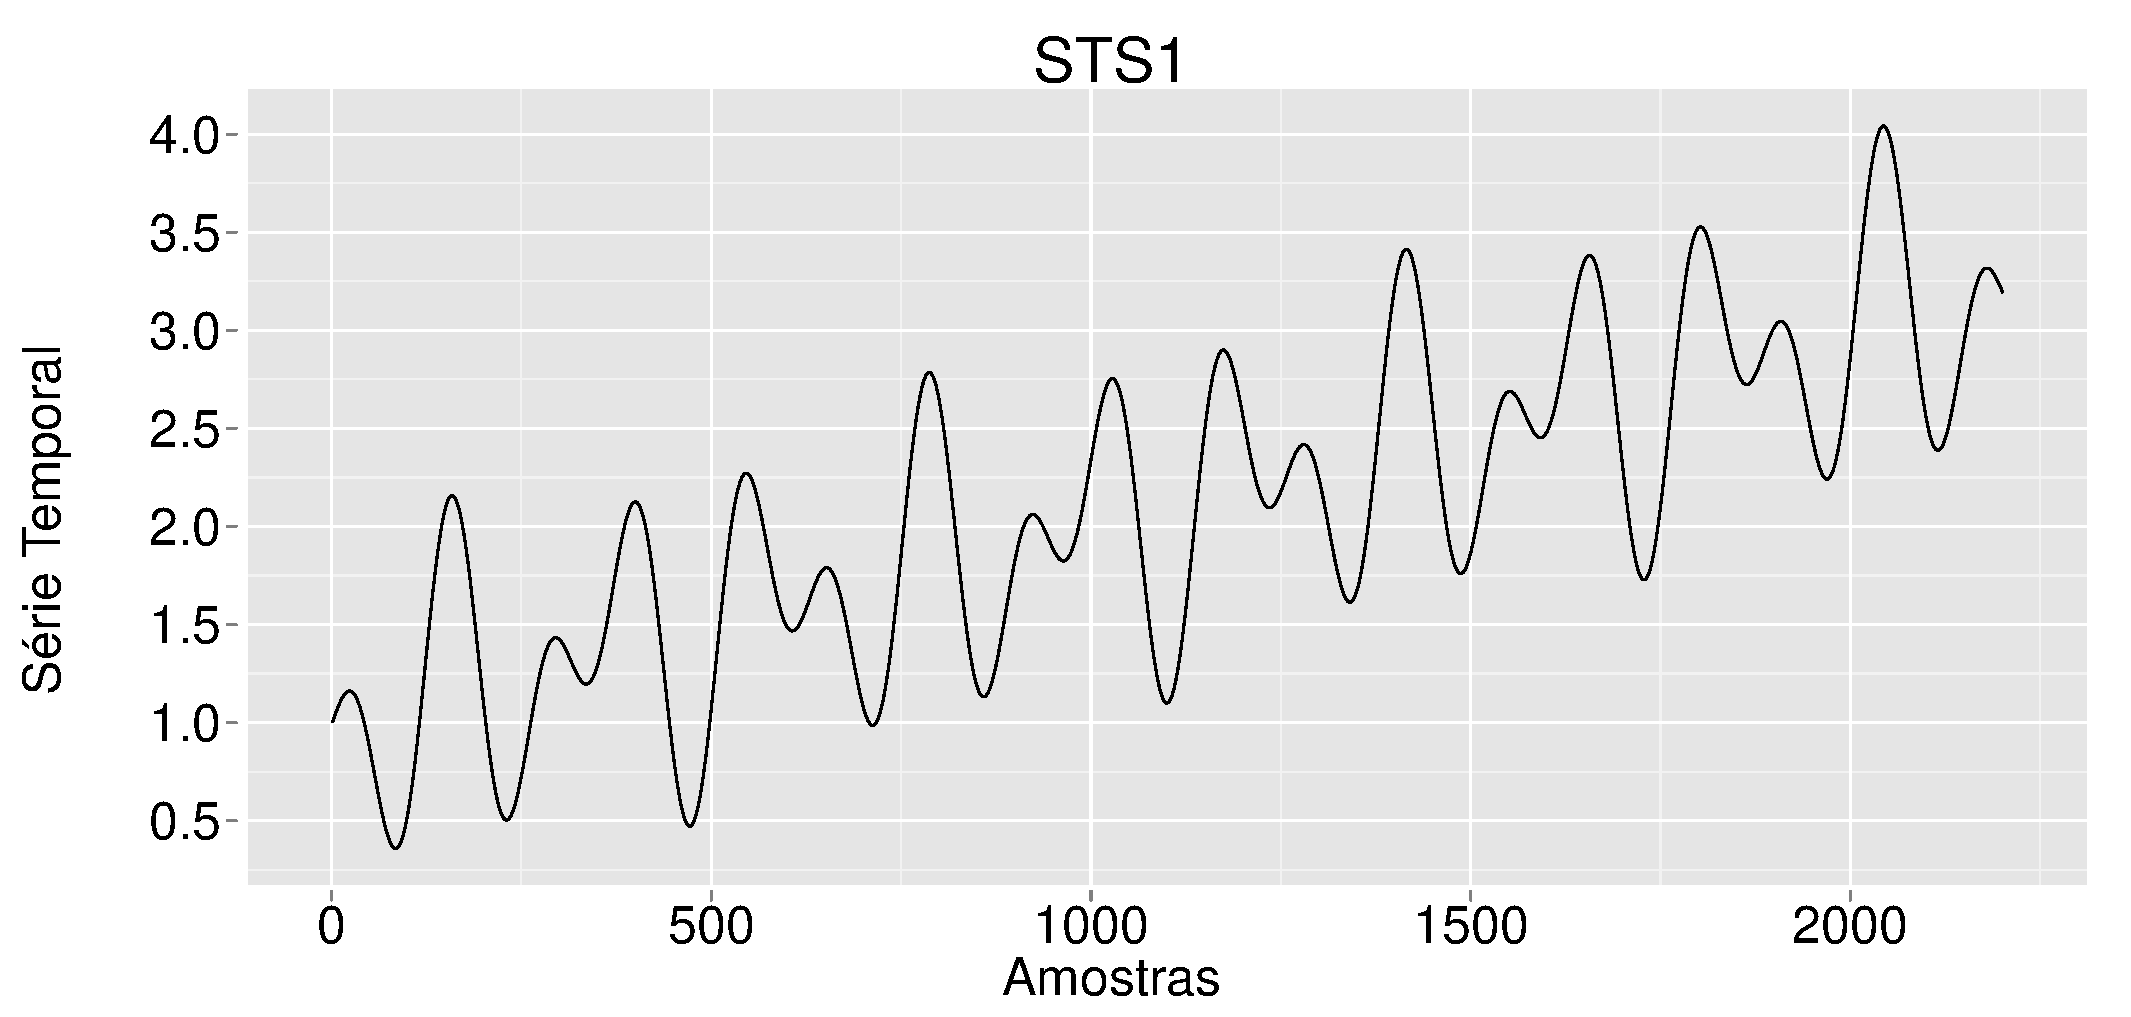
\includegraphics[width=0.49\textwidth]{Cap1/imagens/Arta1.pdf}}
\subfigure[]{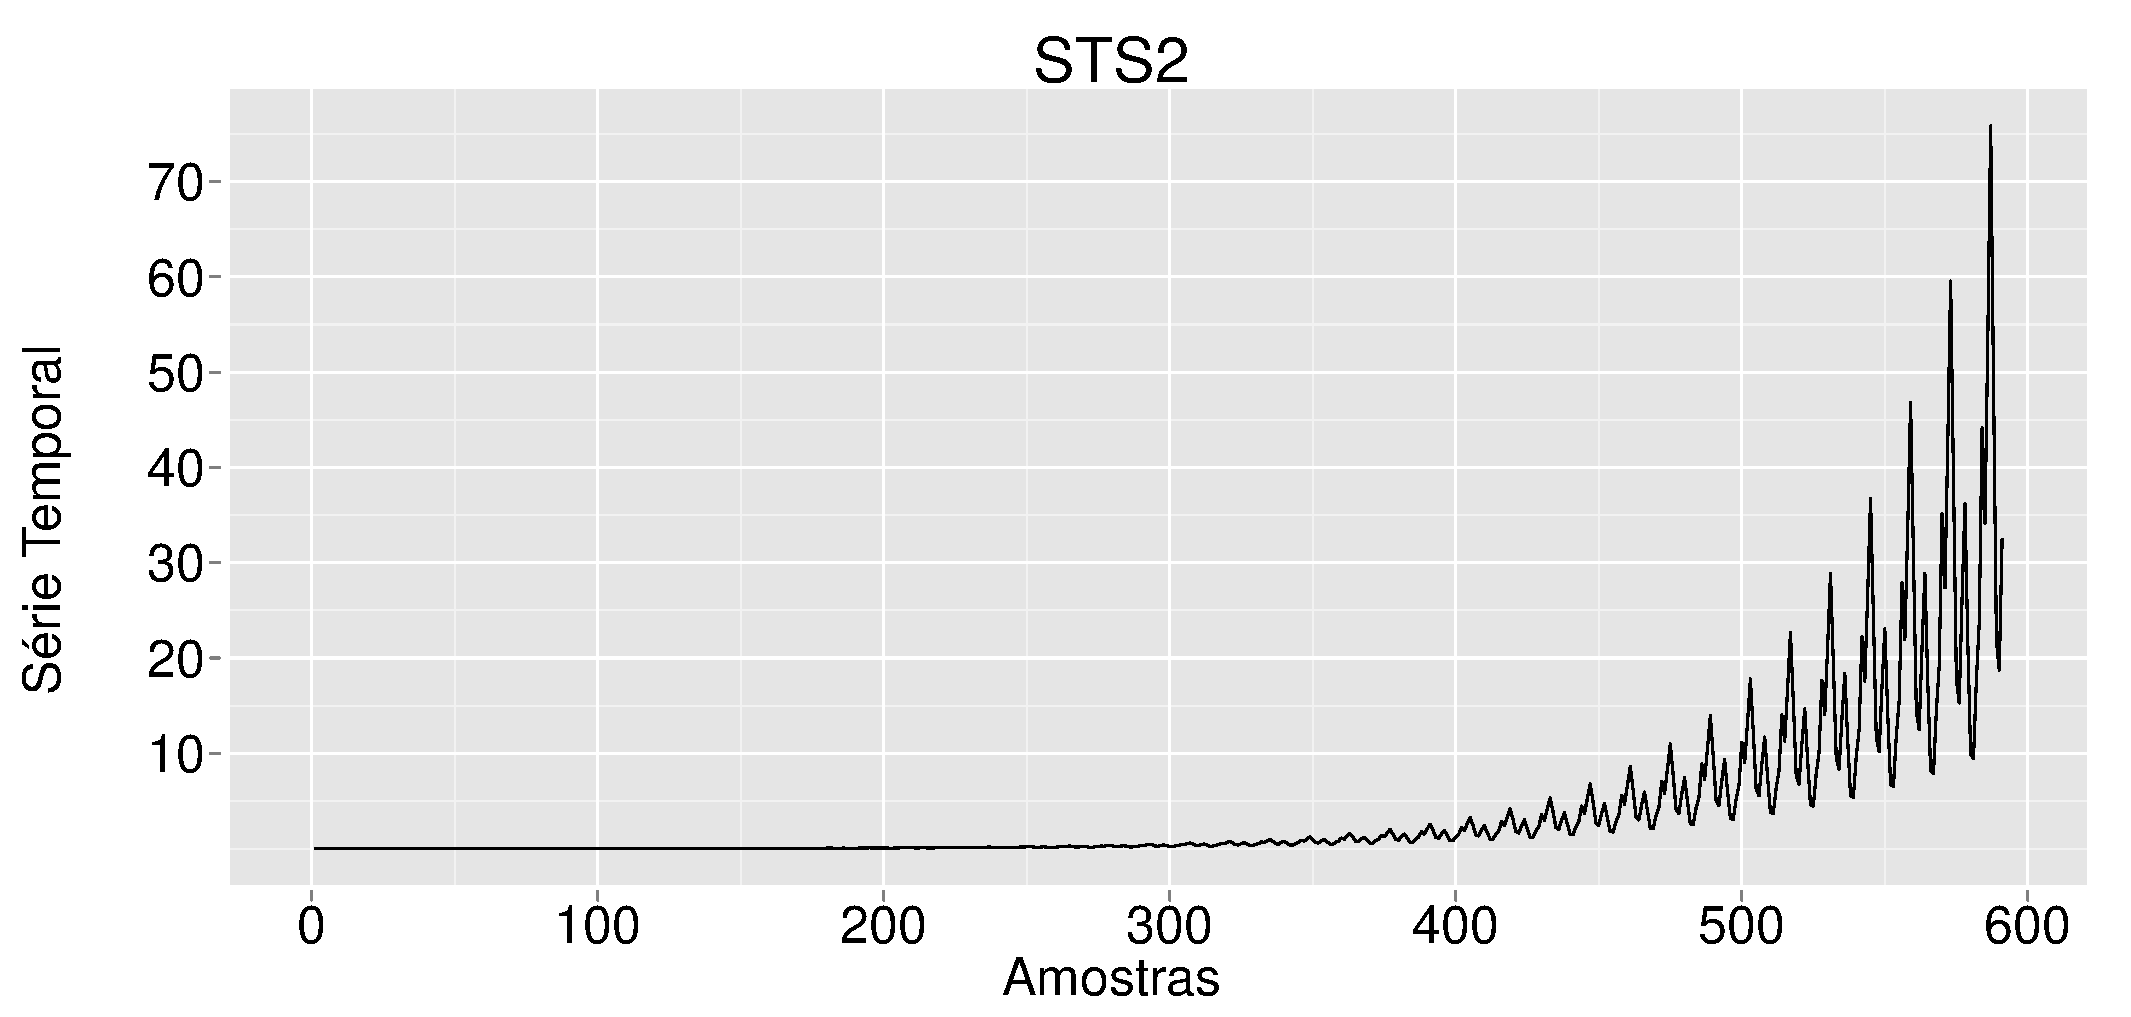
\includegraphics[width=0.49\textwidth]{Cap1/imagens/Arta2.pdf}}
\subfigure[]{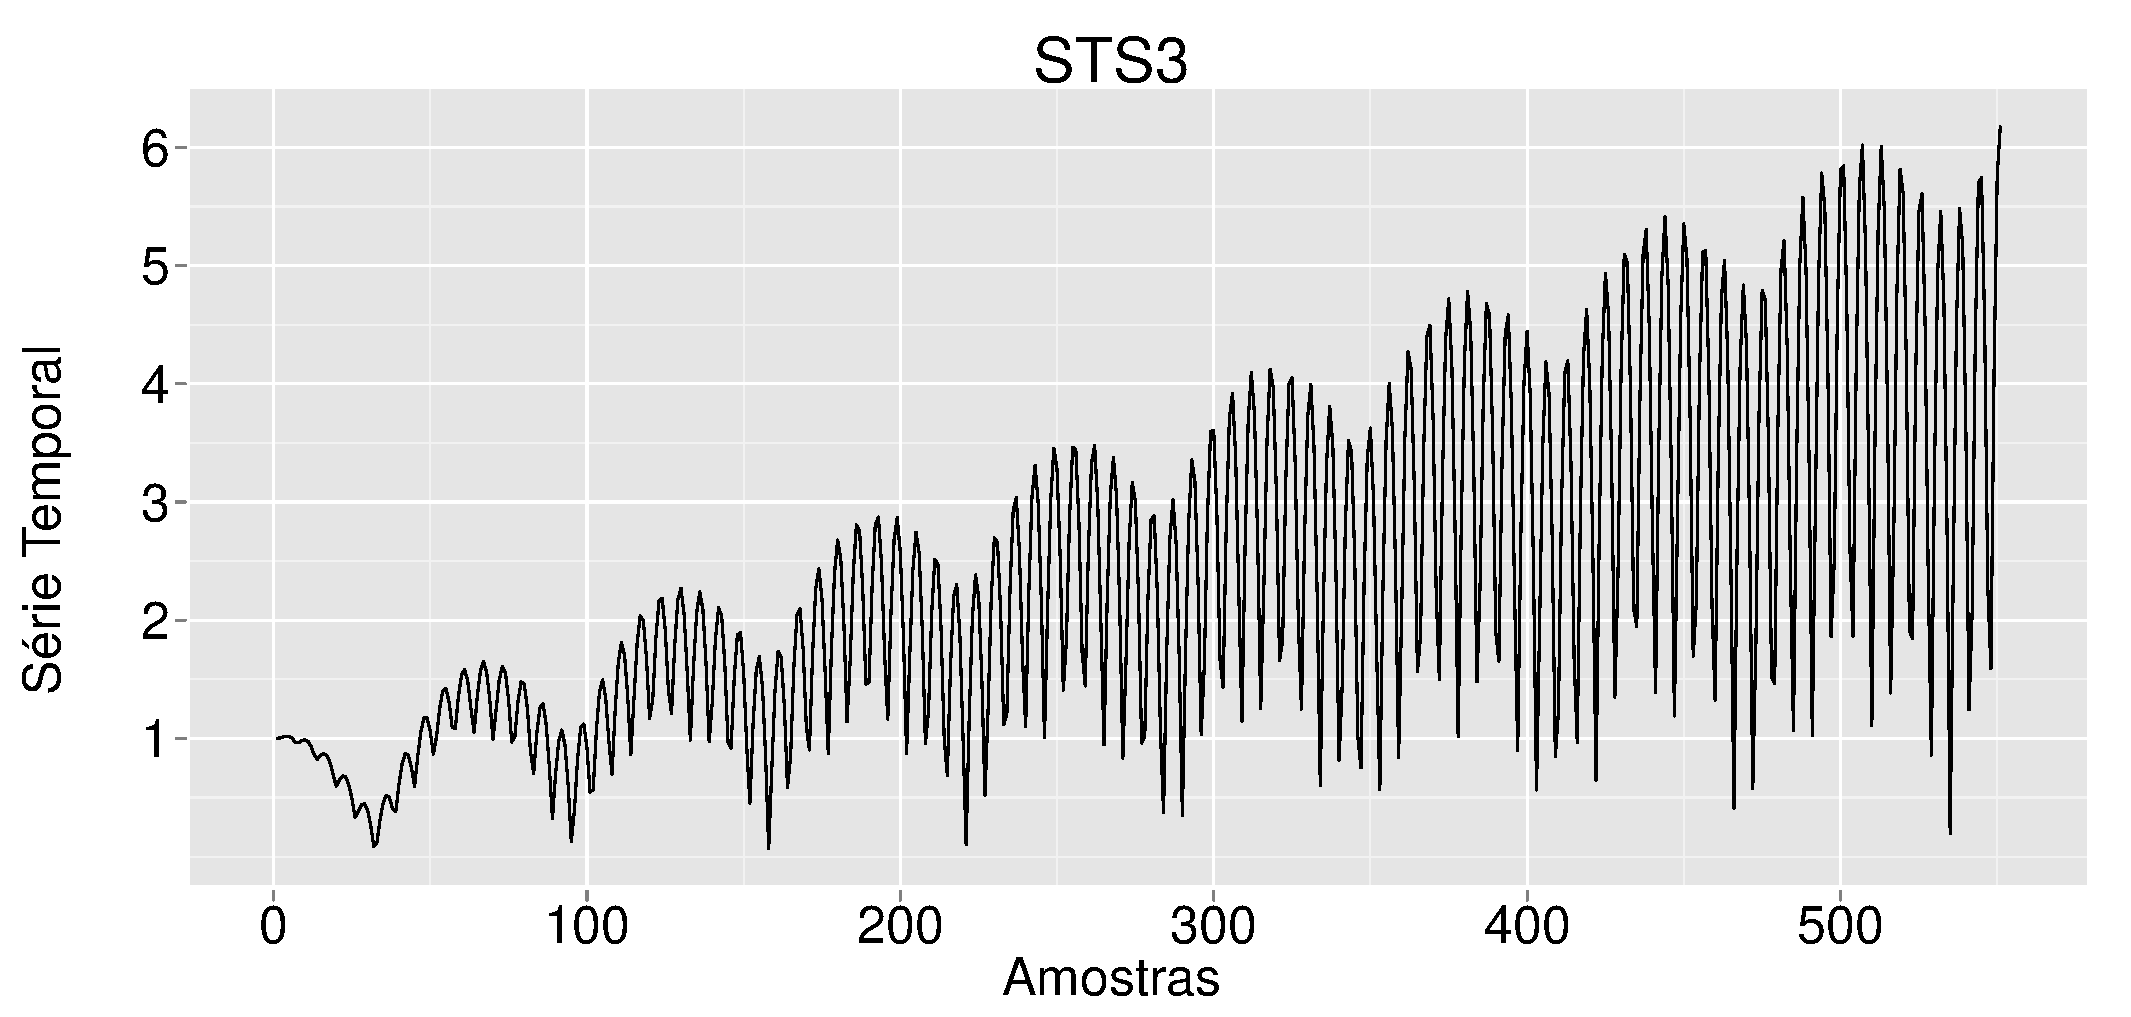
\includegraphics[width=0.49\textwidth]{Cap1/imagens/Arta3.pdf}}
\caption[Séries temporais artificiais geradas através de modelos sazonais]{Séries temporais artificiais geradas através de modelos sazonais: (a) STS1, (b) STS2 e (c) STS3.}
\label{fig:SeriesA}
\end{figure}


Modelo de tabela.
\begin{table}[!htb]
	\centering	
	\label{tab:tab_exemplo}
\begin{tabular}{|c|c|c|}
\hline 
Coluna 1 & Coluna 2 & Coluna 3 \\ 
\hline 
Conteúdo 1 & Conteúdo 2 & Conteúdo 3 \\ 
\hline 
\end{tabular} 
\caption[Texto da lista de tabelas]{Texto abaixo da tabela.}
\end{table}

Exemplo de algoritmo:
No Algoritmo~\ref{alg:kNNTSP}~\cite{Ferrero2009} é apresentado o pseudocódigo, em alto nível, do algoritmo, onde:
\begin{itemize}
\item $Z$ representa a ST utilizada;
\item $w$ representa o tamanho da janela para busca das sequências;
\item $M_s$ representa a medida de similaridade utilizada;
\item $C_k$ representa o critério utilizado para a seleção dos vizinhos próximos;
\item $k$ representa a quantidade de vizinhos mais próximos; e
\item $f$ representa a função de previsão utilizada para o cálculo do valor futuro.
\end{itemize}

\begin{algorithm}[hbtp]
\caption{\textit{$k$-NNTSP}.}
\label{alg:kNNTSP}
\Entrada{$Z$, $w$, $M_s$, $C_k$, $k$, $f$}
\Saida{$\hat{z}_{n+1};$}
\Inicio{
// Construção do conjunto de séries de treinamento $S$ a partir da série temporal $Z$ 

// e tamanho de janela $w$

$S \leftarrow series\_de\_treinamento(Z, w);$

// Definição da sequência de referência $U$

$U \leftarrow (z_n);$

// Obtenção das $k$ sequências mais próximas a $U$ contidas em $S$, considerando a

// medida de similaridade $M_s$ e o critério de seleção de vizinhos próximos $C_k$

$S' \leftarrow vizinhos\_proximos(S, U, M_s, C_k, k);$

// Cálculo do valor futuro da sequências de referências, utilizando $f(S')$

$\hat{z}_{n+1} \leftarrow f(S');$

\Retorna{$\hat{z}_{n+1}$}
}
\end{algorithm}

Exemplo de tabela que ocupa mais de uma página (long tables):

\tablecaption{Características das ST disponíveis pela \textit{NNGC I}.} 
\tablefirsthead{\hline
    \hline
    \multicolumn{1}{c|}{{\scriptsize \textbf{Id}}} & \multicolumn{1}{c|}{{\scriptsize \textbf{Base de Dados}}} & \multicolumn{1}{c|}{{\scriptsize \textbf{Aquisição}}} & \multicolumn{1}{c|}{\scriptsize {\textbf{Tamanho}}} & \multicolumn{1}{c|}{{\scriptsize \textbf{Início }}} & \multicolumn{1}{c}{{\scriptsize \textbf{Término}}} \\
    \hline}
\tablehead{\multicolumn{6}{c}
    {{\tablename\ \thetable{ -- Características das ST disponíveis pela \textit{NNGC I}.}}} \\
    \hline 
    \hline
    \multicolumn{6}{r}
    {\scriptsize Continuação da página anterior.}\\
    \hline
    \multicolumn{1}{c|}{{\scriptsize \textbf{Id}}} & \multicolumn{1}{c|}{{\scriptsize \textbf{Base de Dados}}} & \multicolumn{1}{c|}{{\scriptsize \textbf{Aquisição}}} & \multicolumn{1}{c|}{\scriptsize {\textbf{Tamanho}}} & \multicolumn{1}{c|}{{\scriptsize \textbf{Início }}} & \multicolumn{1}{c}{{\scriptsize \textbf{Término}}}\\}
\tabletail{\hline 
\multicolumn{6}{r}
           {\scriptsize Continua na página seguinte.}\\
            }
\tablelasttail{\hline \hline}
\xentrystretch{-0.15}
\begin{center}
\begin{xtabular}{c|c|c|c|c|c}
    {\scriptsize 1.B-001} & {\scriptsize 1.B}   & {\scriptsize Quaternal} & {\scriptsize 40}   & {\scriptsize jan-1993} & {\scriptsize abr-2002} \\ \hline
    {\scriptsize 1.B-002} & {\scriptsize 1.B}   & {\scriptsize Quaternal} & {\scriptsize 31}   & {\scriptsize jan-1990} & {\scriptsize mar-1997} \\ \hline
    {\scriptsize 1.B-003} & {\scriptsize 1.B}   & {\scriptsize Quaternal} & {\scriptsize 148}   & {\scriptsize jan-1967} & {\scriptsize abr-2003}\\ \hline
    {\scriptsize 1.B-004} & {\scriptsize 1.B}   & {\scriptsize Quaternal} & {\scriptsize 148}   & {\scriptsize jan-1967} & {\scriptsize abr-2003} \\ \hline
    {\scriptsize 1.B-005} & {\scriptsize 1.B}   & {\scriptsize Quaternal} & {\scriptsize 148}   & {\scriptsize jan-1967} & {\scriptsize abr-2003} \\ \hline
    {\scriptsize 1.B-006} & {\scriptsize 1.B}   & {\scriptsize Quaternal} & {\scriptsize 108}   & {\scriptsize jan-1977} & {\scriptsize abr-2003} \\ \hline
    {\scriptsize 1.B-007} & {\scriptsize 1.B}   & {\scriptsize Quaternal} & {\scriptsize 108}   & {\scriptsize jan-1977} & {\scriptsize abr-2003} \\ \hline
    {\scriptsize 1.B-008} & {\scriptsize 1.B}   & {\scriptsize Quaternal} & {\scriptsize 148}   & {\scriptsize jan-1967} & {\scriptsize abr-2003} \\ \hline
    {\scriptsize 1.B-009} & {\scriptsize 1.B}   & {\scriptsize Quaternal} & {\scriptsize 148}   & {\scriptsize jan-1967} & {\scriptsize abr-2003} \\ \hline
    {\scriptsize 1.B-010} & {\scriptsize 1.B}   & {\scriptsize Quaternal} & {\scriptsize 148}   & {\scriptsize jan-1967} & {\scriptsize abr-2003} \\ \hline
    {\scriptsize 1.B-011} & {\scriptsize 1.B}   & {\scriptsize Quaternal} & {\scriptsize 148}   & {\scriptsize jan-1967} & {\scriptsize abr-2003} \\ \hline
    {\scriptsize 1.C-001} & {\scriptsize 1.C}   & {\scriptsize Mensal} & {\scriptsize 48 }   & {\scriptsize jan-1999} & {\scriptsize dez-2002} \\ \hline
    {\scriptsize 1.C-002} & {\scriptsize 1.C}   & {\scriptsize Mensal} & {\scriptsize 48 }   & {\scriptsize jan-1999} & {\scriptsize dez-2002} \\ \hline
    {\scriptsize 1.C-003} & {\scriptsize 1.C}   & {\scriptsize Mensal} & {\scriptsize 198}   & {\scriptsize set-1987} & {\scriptsize fev-2004} \\ \hline
    {\scriptsize 1.C-004} & {\scriptsize 1.C}   & {\scriptsize Mensal} & {\scriptsize 172}   & {\scriptsize jan-1990} & {\scriptsize abr-2004} \\ \hline
    {\scriptsize 1.C-005} & {\scriptsize 1.C}   & {\scriptsize Mensal} & {\scriptsize 118}   & {\scriptsize out-1993} & {\scriptsize jul-2003} \\ \hline
    {\scriptsize 1.C-006} & {\scriptsize 1.C}   & {\scriptsize Mensal} & {\scriptsize 118}   & {\scriptsize out-1993} & {\scriptsize jul-2003} \\ \hline
    {\scriptsize 1.C-007} & {\scriptsize 1.C}   & {\scriptsize Mensal} & {\scriptsize 118}   & {\scriptsize out-1993} & {\scriptsize jul-2003} \\ \hline
    {\scriptsize 1.C-008} & {\scriptsize 1.C}   & {\scriptsize Mensal} & {\scriptsize 57 }   & {\scriptsize abr-1998} & {\scriptsize dez-2002} \\ \hline
    {\scriptsize 1.C-009} & {\scriptsize 1.C}   & {\scriptsize Mensal} & {\scriptsize 227}   & {\scriptsize jan-1983} & {\scriptsize nov-2001} \\ \hline
    {\scriptsize 1.C-010} & {\scriptsize 1.C}   & {\scriptsize Mensal} & {\scriptsize 132}   & {\scriptsize abr-1993} & {\scriptsize mar-2004} \\ \hline
    {\scriptsize 1.C-011} & {\scriptsize 1.C}   & {\scriptsize Mensal} & {\scriptsize 228}   & {\scriptsize mar-1986} & {\scriptsize fev-2005} \\ \hline
    {\scriptsize 1.D-001} & {\scriptsize 1.D}   & {\scriptsize Semanal} & {\scriptsize 527 }  & {\scriptsize 02-jan-1995} & {\scriptsize 31-jan-2005} \\ \hline
    {\scriptsize 1.D-003} & {\scriptsize 1.D}   & {\scriptsize Semanal} & {\scriptsize 437 }  & {\scriptsize 03-jan-1997} & {\scriptsize 13-mai-2005} \\ \hline
    {\scriptsize 1.D-004} & {\scriptsize 1.D}   & {\scriptsize Semanal} & {\scriptsize 549 }  & {\scriptsize 11-nov-1994} & {\scriptsize 13-mai-2005} \\ \hline
    {\scriptsize 1.D-005} & {\scriptsize 1.D}   & {\scriptsize Semanal} & {\scriptsize 437 }  & {\scriptsize 03-jan-1997} & {\scriptsize 13-mai-2005} \\ \hline
    {\scriptsize 1.D-006} & {\scriptsize 1.D}   & {\scriptsize Semanal} & {\scriptsize 618 }  & {\scriptsize 16-jul-1993} & {\scriptsize 13-mai-2005} \\ \hline
    {\scriptsize 1.D-007} & {\scriptsize 1.D}   & {\scriptsize Semanal} & {\scriptsize 618 }  & {\scriptsize 16-jul-1993} & {\scriptsize 13-mai-2005} \\ \hline
    {\scriptsize 1.D-008} & {\scriptsize 1.D}   & {\scriptsize Semanal} & {\scriptsize 548 }  & {\scriptsize 18-nov-1994} & {\scriptsize 13-mai-2005} \\ \hline
    {\scriptsize 1.D-009} & {\scriptsize 1.D}   & {\scriptsize Semanal} & {\scriptsize 548 }  & {\scriptsize 18-nov-1994} & {\scriptsize 13-mai-2005} \\ \hline
    {\scriptsize 1.D-010} & {\scriptsize 1.D}   & {\scriptsize Semanal} & {\scriptsize 593 }  & {\scriptsize 07-jan-1994} & {\scriptsize 13-mai-2005} \\ \hline
    {\scriptsize 1.D-011} & {\scriptsize 1.D}   & {\scriptsize Semanal} & {\scriptsize 594 }  & {\scriptsize 10-jan-1994} & {\scriptsize 23-mai-2005} \\ \hline
    {\scriptsize 1.E-001} & {\scriptsize 1.E}   & {\scriptsize Diária} & {\scriptsize 377}   & {\scriptsize 01-jan-2005} & {\scriptsize 12-jan-2006} \\ \hline
    {\scriptsize 1.E-002} & {\scriptsize 1.E}   & {\scriptsize Diária} & {\scriptsize 377}   & {\scriptsize 01-jan-2005} & {\scriptsize 12-jan-2006} \\ \hline
    {\scriptsize 1.E-004} & {\scriptsize 1.E}   & {\scriptsize Diária} & {\scriptsize 466}   & {\scriptsize 07-fev-2003} & {\scriptsize 17-mai-2004} \\ \hline
    {\scriptsize 1.E-005} & {\scriptsize 1.E}   & {\scriptsize Diária} & {\scriptsize 716}   & {\scriptsize 01-jan-2002} & {\scriptsize 17-dez-2003} \\ \hline
    {\scriptsize 1.E-006} & {\scriptsize 1.E}   & {\scriptsize Diária} & {\scriptsize 502}   & {\scriptsize 01-jan-2002} & {\scriptsize 17-mai-2003} \\ \hline
    {\scriptsize 1.E-007} & {\scriptsize 1.E}   & {\scriptsize Diária} & {\scriptsize 502}   & {\scriptsize 01-jan-2002} & {\scriptsize 17-mai-2003} \\ \hline
    {\scriptsize 1.E-008} & {\scriptsize 1.E}   & {\scriptsize Diária} & {\scriptsize 747}   & {\scriptsize 01-nov-2003} & {\scriptsize 16-nov-2005} \\ \hline
    {\scriptsize 1.E-009} & {\scriptsize 1.E}   & {\scriptsize Diária} & {\scriptsize 747}   & {\scriptsize 01-nov-2003} & {\scriptsize 16-nov-2005} \\ \hline
    {\scriptsize 1.E-010} & {\scriptsize 1.E}   & {\scriptsize Diária} & {\scriptsize 654}   & {\scriptsize 01-jul-2003} & {\scriptsize 14-abr-2005} \\ \hline
    {\scriptsize 1.E-011} & {\scriptsize 1.E}   & {\scriptsize Diária} & {\scriptsize 654}   & {\scriptsize 01-jul-2003} & {\scriptsize 14-abr-2005} \\ \hline
    {\scriptsize 1.F-003} & {\scriptsize 1.F}   & {\scriptsize Horária (5:00-24:00)} & {\scriptsize 1742}  & {\scriptsize 02-jan-2005} & {\scriptsize 29-mar-2005} \\ \hline
    {\scriptsize 1.F-004} & {\scriptsize 1.F}   & {\scriptsize Horária (5:00-24:00)} & {\scriptsize 902 }  & {\scriptsize 05-set-2005} & {\scriptsize 19-out-2005} \\ \hline
    {\scriptsize 1.F-005} & {\scriptsize 1.F}   & {\scriptsize Horária (5:00-24:00)} & {\scriptsize 902 }  & {\scriptsize 05-set-2005} & {\scriptsize 19-out-2005} \\ \hline
    {\scriptsize 1.F-006} & {\scriptsize 1.F}   & {\scriptsize Horária (5:00-24:00)} & {\scriptsize 1742}  & {\scriptsize 02-jan-2005} & {\scriptsize 29-mar-2005} \\ \hline
    {\scriptsize 1.F-007} & {\scriptsize 1.F}   & {\scriptsize Horária (5:00-24:00)} & {\scriptsize 1742}  & {\scriptsize 02-jan-2005} & {\scriptsize 29-mar-2005} \\ \hline
    {\scriptsize 1.F-008} & {\scriptsize 1.F}   & {\scriptsize Horária (5:00-24:00)} & {\scriptsize 1742}  & {\scriptsize 02-jan-2005} & {\scriptsize 29-mar-2005} \\ \hline
    {\scriptsize 1.F-009} & {\scriptsize 1.F}   & {\scriptsize Horária (5:00-24:00)} & {\scriptsize 902 }  & {\scriptsize 05-set-2005} & {\scriptsize 19-out-2005} \\ \hline
    {\scriptsize 1.F-010} & {\scriptsize 1.F}   & {\scriptsize Horária (5:00-24:00)} & {\scriptsize 902 }  & {\scriptsize 05-set-2005} & {\scriptsize 19-out-2005} \\ \hline
    {\scriptsize 1.F-011} & {\scriptsize 1.F}   & {\scriptsize Horária (5:00-24:00)} & {\scriptsize 902 }  & {\scriptsize 05-set-2005} & {\scriptsize 19-out-2005} \\ 
\end{xtabular}
\end{center}





\chapter{Revisão Bibliográfica}\label{ch:rev_bib}


\chapter{Metodologia}\label{ch:metodologia}

\chapter{Implementaç\~ao}\label{ch:implementacao}

\chapter{Resultados}\label{ch:resultados}


\chapter{Conclus\~ao}\label{ch:conclusao}


%---------- Referencias ----------
\flushleft

\bibliography{tccNovo.bib} % geracao automatica das referencias a partir do arquivo reflatex.bib

\end{document}
